\chapter{Extensions}
\label{section:extensions}

\section{Solver-specific Improvements}
The main principles that drive the algorithm work regardless of which solver is used. However, the implementation can be improved by using more specific features of the solver. For this thesis, IBM CPLEX is used as the MILP solver. This is one of the fastest, proprietary solvers available on the market. 

\subsection{Indicator Constraints}
The Big M method, used to turn constraints on or off, is functional, but there are some issues with it. The value of M has to be large enough so it can always overpower the rest of the inequality. If M is too small, incorrect behavior may occur. However, if M is very large, CPLEX may have numerical difficulties or even find incorrect results \footnote{\url{http://www-01.ibm.com/support/docview.wss?uid=swg21400084}}.
\par
Indicator constraints are a solution for this problem. The goal of the large M is to overpower the inequality so the constraint can be turned on or off based on a boolean variable. Indicator constraints allow constraints to be turned on or off, based on other constraints. They provide a direct way to model an "if/then" relation. Equation \ref{eq:indicator-obs} is a modified version of the obstacle avoidance constraints \ref{eq:obs-m-1-v} - \ref{eq:obs-m-4-v}. If $slack_{i,n}$ is not true, then the matching constraint on the right side must be true.

\begin{equation}
\label{eq:indicator-obs}
\neg slack_{i,n} \rightarrow \\
\begin{cases}
y_{n} -  o_i \quad \geq 
\quad a_{i} x_{n} + b_{i},  	
& \Delta q_{x,i} < 0 							 	
 \\
y_{n} + o_i \quad \leq 
\quad a_{i} x_{n} + b_{i},
& \Delta q_{x,i} > 0 							 	
 \\
x_{n} + r \quad \leq
\quad  q_{x,i}, 		
& \Delta q_{y,i} < 0, \quad \Delta q_{x,i} = 0 	
 \\
x_{n} - r \quad \geq 
\quad q_{y,i},  		
& \Delta q_{y,i} > 0, \quad \Delta q_{x,i} = 0 	
\end{cases}
\end{equation}

\subsection{Maximum Solve Time}
When the MILP problem is sufficiently difficult to solve, it may take a long time before the solver can find the optimal solution. To ensure an upper limit on computation time, CPLEX accepts a maximum solve time parameter. When the maximum time has expired, it will return the best solution found so far.
\par
In the experiments, the maximum solve time was typically 120 seconds per segment. The goal is for every segment to be relatively easy to solve, so if no solution can be found in two minutes it counts as a failure.
\subsection{Maximum Solution Delta}
During testing it became clear that the solver often spends a relatively long time trying to improve trajectories which are already nearly optimal, or optimal but not yet proven to be optimal. CPLEX provides a maximum delta parameter. The delta is the difference between the best solution found so far and the upper bound for the optimal solution. If the delta is below this maximum delta, the solvers stop executing and returns the best result. When this value is small, this can reduce some of the execution time while barely changing the quality of the trajectory.

\section{Corner Cutting Prevention}
\label{subsec:corner-cutting}
\begin{figure}
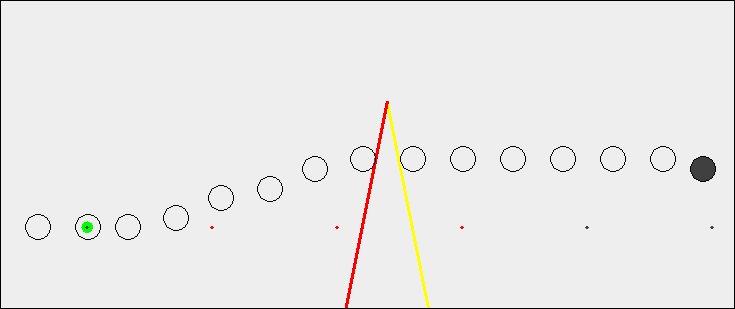
\includegraphics[width=\textwidth]{img/cornercut_bad}
\caption{An example of corner cutting}
\label{fig:cornercut-example}
\end{figure}
The MILP problem uses discrete time steps to model the changes in the UAV's state over time. An issue with this approach is that constraints are only enforced at those specific time steps. This allows the UAV to cut corners or even move through obstacles entirely if the vehicle is moving fast enough. Figure \ref{fig:cornercut-example} shows an example of this. Each time step on its own is a valid position, but a collision is ignored between the time steps.
\par
Using the indicator constraint notation, Equation \ref{eq:obs-repeat-1} and \ref{eq:obs-comb-repeat-1} prevent collisions with an obstacle at time step $n$. Each edge of the obstacle has an associated $slack$ variable, which determines whether or not the UAV is on the safe side for that edge.
\begin{equation}
\label{eq:obs-repeat-1}
\neg ~ slack_{i,n} \rightarrow \\
\begin{cases}
y_{n} -  o_i \quad \geq 
\quad a_{i} x_{n} + b_{i},  	
& \Delta q_{x,i} < 0 							 	
 \\
y_{n} + o_i \quad \leq 
\quad a_{i} x_{n} + b_{i},
& \Delta q_{x,i} > 0 							 	
 \\
x_{n} + r \quad \leq
\quad  q_{x,i}, 		
& \Delta q_{y,i} < 0, \quad \Delta q_{x,i} = 0 	
 \\
x_{n} - r \quad \geq 
\quad q_{y,i},  		
& \Delta q_{y,i} > 0, \quad \Delta q_{x,i} = 0 	
\end{cases}
\end{equation}
\begin{equation}
\label{eq:obs-comb-repeat-1}
\neg \mathlarger{\mathlarger{\bigwedge_{i}}} slack_{i,n} \quad 0 \leq n \leq N
\end{equation}
Richards and Turnbull\cite{Richards2015} proposed a method which prevents corner cutting. In their method, the UAV is considered on the safe side of an edge only if that is true for two consecutive time steps.  This is visualized in Figure \ref{fig:cc-fixed}. They apply the same constraints again, but this time on the position of the UAV in the last time step. Equation \ref{eq:corner-skip-fixed} expresses this requirement:
\begin{equation}
\label{eq:corner-skip-fixed}
\neg ~ slack_{i,n} \rightarrow \\
\begin{cases}
y_{n-1} -  o_i \quad \geq 
\quad a_{i} x_{n-1} + b_{i},  	
& \Delta q_{x,i} < 0 							 	
 \\
y_{n-1} + o_i \quad \leq 
\quad a_{i} x_{n-1} + b_{i},
& \Delta q_{x,i} > 0 							 	
 \\
x_{n-1} + r \quad \leq
\quad  q_{x,i}, 		
& \Delta q_{y,i} < 0, \quad \Delta q_{x,i} = 0 	
 \\
x_{n-1} - r \quad \geq 
\quad q_{y,i},  		
& \Delta q_{y,i} > 0, \quad \Delta q_{x,i} = 0 	
\end{cases}
\end{equation}
\begin{figure}
	\centering
	\begin{subfigure}[t]{0.3\columnwidth}
        		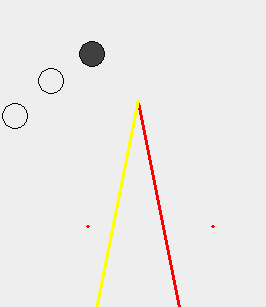
\includegraphics[width=\textwidth]{cornercut-fixed-1}
        		\caption{}
        		\label{fig:cc-fixed-1}
	\end{subfigure}
	\hfil
	\begin{subfigure}[t]{0.3\columnwidth}
        		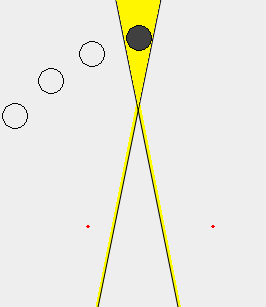
\includegraphics[width=\textwidth]{cornercut-fixed-2b}
        		\caption{}
        		 \label{fig:cc-fixed-2}
	\end{subfigure}	
		\hfil
	\begin{subfigure}[t]{0.3\columnwidth}
        		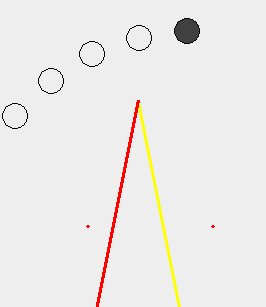
\includegraphics[width=\textwidth]{cornercut-fixed-3}
        		\caption{}
        		\label{fig:cc-fixed-3}
	\end{subfigure}
    \caption[A visual demonstration of how the corner cutting prevention works.]{These figures show three consecutive time steps which demonstrate how the corner cutting prevention works. In \ref{fig:cc-fixed-1}, the UAV is in the safe region of the left edge (which is indicated by the yellow color). In \ref{fig:cc-fixed-3}, the UAV is in the safe region for the right edge, but not the left edge. To ensure that the UAV does not cut the corner, the UAV must enter the safe region of the right edge before it exits the safe region of the left edge. The intersection between those two safe regions is the inverted yellow triangle in \ref{fig:cc-fixed-2}. If the UAV spends at least one time step in that yellow, it cannot cut the corner.}
    \label{fig:cc-fixed}     
\end{figure}

\section{Goal Conditions}
\label{subsec:goal-cond}

\begin{figure}
	\centering
	\begin{subfigure}[t]{0.45\columnwidth}
        		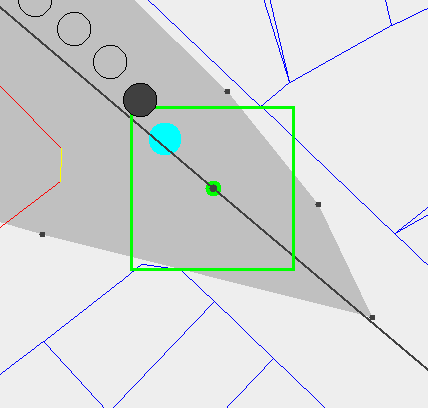
\includegraphics[width=\textwidth]{segment-pre-goal-zoom}
        		\caption{}
        		 \label{fig:goal-ext-pre}
	\end{subfigure}	
		\hfil
	\begin{subfigure}[t]{0.45\columnwidth}
        		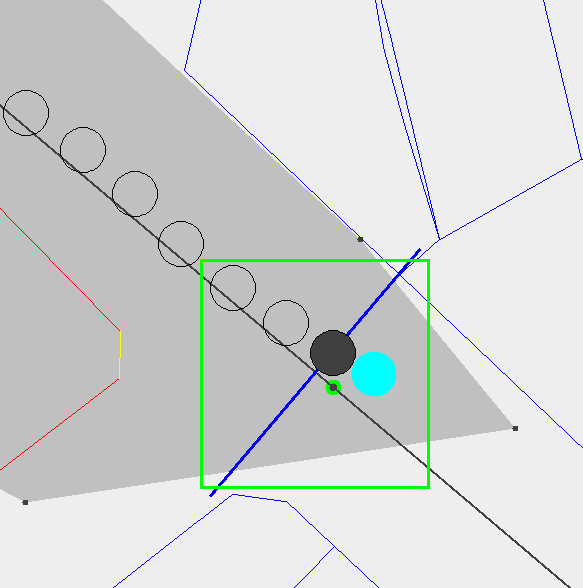
\includegraphics[width=\textwidth]{segment-extend-goal-zoom}
        		\caption{}
        		\label{fig:goal-ext-post}
	\end{subfigure}
    \caption[A visualization of the extended goal conditions]{\ref{fig:goal-ext-pre} shows the UAV right before reaching its goal. The blue circle shows the position of the UAV at the segment transition. The goal position is the green dot, while the square around it shows the tolerance region where the goal is considered to be reached. Note how the segment transition happens earlier because of the tolerance region. \ref{fig:goal-ext-post} shows the same, only this time a (blue) finish line is added. This time, the UAV needs to cross the finish line so the segment transition is roughly as far along the path as planned.}
    \label{fig:goal-ext}     
\end{figure}
Forcing the UAV to exactly reach each intermediate goal position is overly restrictive. Because the goal conditions are only checked for each time step, the arrival at the goal position must line up with a time step. If this is not the case, the UAV could be right before the goal position on one time step, and already have passed the goal position by the next time step. The result is that the UAV will slow down near the end of each segment so it can exactly line up with the goal position for that segment. This effect gets worse as the velocity increases.
\par
By allowing some difference between the goal position and the position of the UAV, this behavior can be resolved. However, this tolerance on the UAV's position means that the goal condition tends to be satisfied before the UAV has actually reached the goal. This is visible in Figure \ref{fig:goal-ext-pre}. By adding a finish line perpendicular to the path at the goal position and forcing the UAV to cross this line, this early finish can be counteracted. The tolerance makes the trajectory less restricted, while the finish line ensures that the segment transitions happen at the right time. This can be seen in Figure \ref{fig:goal-ext-post}.
\newpage
\section{Stability Improvements}

\subsection{Maximum Goal Velocity}
\label{subsec:maxgoalvel}
\begin{figure}[]
	\centering
	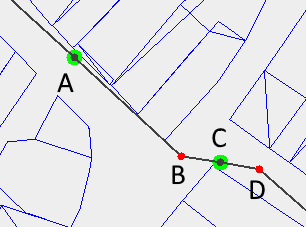
\includegraphics[width=0.5\textwidth]{goalvel}
	\caption[A scenario in which a maximum goal velocity is useful.]{A visual demonstration of when a maximum goal velocity is used. Points B and D are individual turn events. The segment for event B starts at A, with $|AB|$ being the desired expansion distance for the segment. However, because D is so close to B, the end of the first segment (at C) cannot be placed at the desired expansion distance from B. Instead, C is placed in the middle between B and D, such that $|BC|=|CD|$. The first segment solves the trajectory from A to C past turn event B, the second segment starts as C, past D and onwards. The goal is to ensure that the UAV can still safely stop at D when it starts the second segment at C. This is done by limiting the maximum velocity of the UAV when it reaches the goal C in the first segment.}
	\label{fig:max-goal-vel}
\end{figure}

When two turn events are close to each other, it may not be possible to expand each corner outwards by the full expansion distance. In that case, the middle between those turn events is chosen as the transition between the the segments.
\par
This ensures that both segments get a fair share of the space between them. However, it breaks the assumption behind the expansion distance around turn events. If the velocity after the first segment is high, due to the reduced approach distance, the UAV may not be able to stop in time to avoid a collision in the next segment. In this situation, no solution will be found in the second segment. Figure \ref{fig:max-goal-vel} shows a situation when this may be necessary.
\par
As a solution for this, the UAVs velocity at the goal of the first segment can be limited so it can stop in time for the turn event in the next segment. The maximum distance at the goal of the segment is $v'_{max}$, given the actual expansion distance $dist$ in Equation \ref{eq:goalvel}. 
\begin{equation}
\label{eq:goalvel}
v'_{max} = \sqrt{2 * dist * a_{max}}
\end{equation}

\subsection{Initial Safe Region}
\label{subsec:safe-ext}
\begin{figure}
	\centering
	\begin{subfigure}[t]{0.35\columnwidth}
        		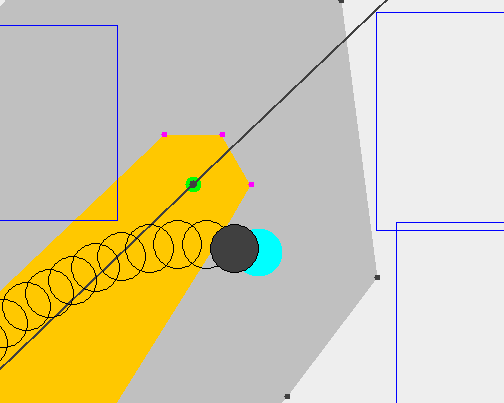
\includegraphics[width=\textwidth]{stoppoint-fail-pre}
        		\caption{}
        		\label{fig:stoppoint-fail-pre}
	\end{subfigure}
	\hfill
	\begin{subfigure}[t]{0.35\columnwidth}
        		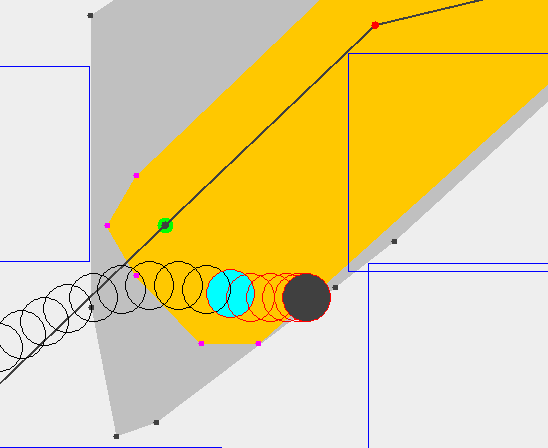
\includegraphics[width=\textwidth]{stoppoint-fail-post}
        		\caption{}
        		 \label{fig:stoppoint-fail-post}
	\end{subfigure}		
	\caption[A case in which a lack of stop point makes a segment transition fail]{An example of how the transition between segments can fail. In \ref{fig:stoppoint-fail-pre}, shows the UAV right before the segment transition, which happens at the blue circle. \ref{fig:stoppoint-fail-post} shows the orange initial safe region and dark grey expanded safe region of the next segment, after the transition. The next segment fails to solve because the UAV cannot come to a stop within the safe region. The position of the UAV shows where the UAV came to a stop in the previous segment (the safe region of which is the grey region in \ref{fig:stoppoint-fail-pre}).}
    \label{fig:stoppoint-fail}     
\end{figure}

The genetic algorithm is relatively simple and makes no attempt to construct the safe region such that the UAV can always stay inside it. This is problematic when the UAV has a long maximum acceleration distance. This problem presents itself in two ways.
\par
The first issue arises at the start of the segment. The maximum goal velocity from section \ref{subsec:maxgoalvel} limits the UAV's velocity, but it does not determine which way the vector is pointed. The maximum goal velocity only ensures safety when the velocity vector is pointed along the path. If the velocity vector is not pointed entirely along the path, the UAV may not be able to stay within the safe region generated by the genetic algorithm. This can be seen in Figure \ref{fig:stoppoint-fail}. The solution for this issue is including the "stop point" in the initial set of points used for the safe region. This stop point is the position where the UAV would come to a halt if it starts to decelerate at the start of the segment. This depends on the initial velocity vector for that segment.
\par
\begin{figure}
	\centering
	\begin{subfigure}[t]{0.30\columnwidth}
        		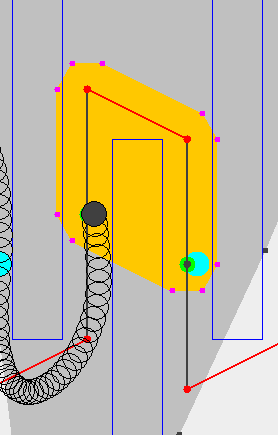
\includegraphics[width=\textwidth]{limited-ga-seed-1}
        		\caption{}
        		\label{fig:ga-seed-without}
	\end{subfigure}
	\hfill
	\begin{subfigure}[t]{0.30\columnwidth}
        		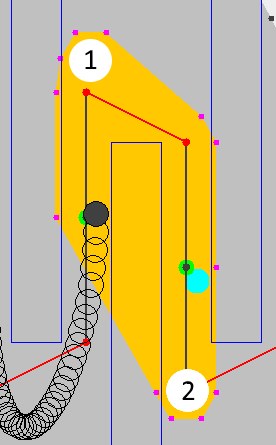
\includegraphics[width=\textwidth]{extended-ga-seed-2}
        		\caption{}
        		 \label{fig:ga-seed-with}
	\end{subfigure}	
	\hfill
	\begin{subfigure}[t]{0.30\columnwidth}
        		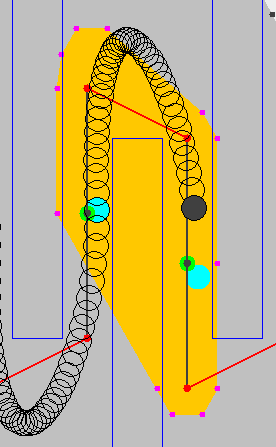
\includegraphics[width=\textwidth]{extended-ga-seed-2b}
        		\caption{}
        		 \label{fig:ga-seed-nomaxvela}
	\end{subfigure}		
	\caption[The effect of the inclusion of stop points on the initial convex safe region.]{\ref{fig:ga-seed-without} shows the initial safe region without the extra stop points in orange. \ref{fig:ga-seed-with} shows the initial safe region with the extra stop points. The position marked with "1" is the stop point for the initial velocity, while the position marked with "2" is the stop point for the trajectory after the goal has been reached. \ref{fig:ga-seed-nomaxvela} shows how the stop point ensured that the UAV could stop. The UAV leaves the initial safe region because it already has started to turn, however the stop point clearly provided enough space.}
    \label{fig:ga-seed-1}     
\end{figure}
The second issue comes into play at the end of a segment. The sub-trajectory for each segment does not end when the goal is reached. It must be calculated for all available time steps. The safe region may be very restrictive just after the UAV has reached its goal. The result is that the UAV has to slow down \emph{before} it reaches its goal to ensure that the rest of the trajectory stays within the safe region. This can also by counteracted by including a stop point in the safe region. This time, the velocity vector of the UAV is not known in advance (since the segment has not been solved yet). The velocity vector is assumed to point along the path and the magnitude is either the maximum goal velocity or maximum velocity, depending on whether the maximum goal velocity is defined.
\par

\begin{figure}
	\centering
	\begin{subfigure}[t]{0.30\columnwidth}
        		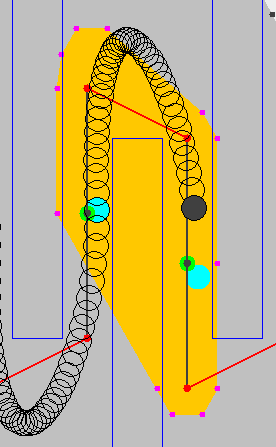
\includegraphics[width=\textwidth]{extended-ga-seed-2b}
        		\caption{}
        		 \label{fig:ga-seed-nomaxvelb}
	\end{subfigure}	
	\hfill
	\begin{subfigure}[t]{0.30\columnwidth}
        		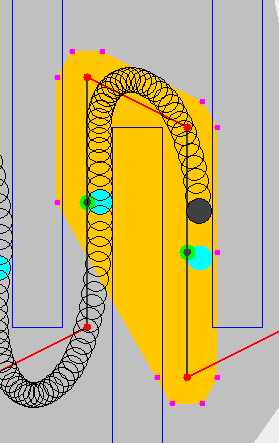
\includegraphics[width=\textwidth]{extended-ga-seed-2c}
        		\caption{}
        		 \label{fig:ga-seed-maxvelc}
	\end{subfigure}		
	\caption[A demonstration of why stop points should only be used with a maximum goal velocity.]{ \ref{fig:ga-seed-nomaxvelb} and \ref{fig:ga-seed-maxvelc} show the trajectory respectively without and with the maximum goal velocity enabled. In \ref{fig:ga-seed-nomaxvelb}, the UAV overshoots the corner which results in a slower trajectory.}
    \label{fig:ga-seed-maxvel}     
\end{figure}

\clearpage

Figure \ref{fig:ga-seed-1} shows the result when both of these stop points are included. In the example, the maximum goal velocity has been ignored to exaggerate the effect. However, the extra stop points should always be used together with the maximum goal velocity. The stop points allow the UAV to make the transition between segments at higher velocities, but that also means they can overshoot in turns. This is demonstrated in Figure \ref{fig:ga-seed-maxvel}.

\begin{figure}[h]
	\centering
	\begin{subfigure}[t]{0.30\columnwidth}
        		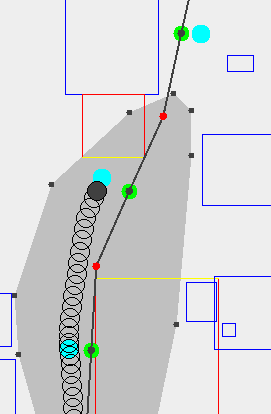
\includegraphics[width=\textwidth]{img/transition-suboptimal-pre}
        		\caption{}
        		 \label{fig:transition-suboptimal-pre}
	\end{subfigure}	
	\hfill
	\begin{subfigure}[t]{0.30\columnwidth}
        		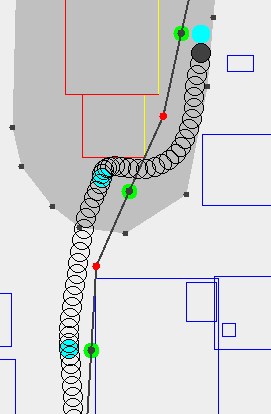
\includegraphics[width=\textwidth]{img/transition-suboptimal-post}
        		\caption{}
        		 \label{fig:transition-suboptimal-post}
	\end{subfigure}	
		\hfill
	\begin{subfigure}[t]{0.30\columnwidth}
        		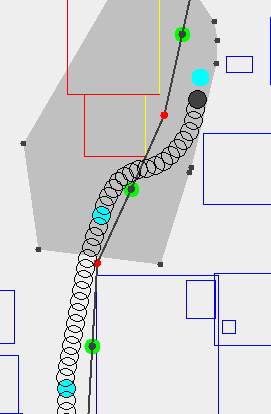
\includegraphics[width=\textwidth]{img/transition-suboptimal-fixed}
        		\caption{}
        		 \label{fig:transition-suboptimal-fixed}
	\end{subfigure}		
	\caption[A case in which overlapping segments significantly improves the quality of the trajectory]{\ref{fig:transition-suboptimal-pre} shows the optimal approach to the goal of the previous segment. However, as seen in \ref{fig:transition-suboptimal-post}, this is a very bad start state for the next segment. By starting the next segment 5 time steps earlier in \ref{fig:transition-suboptimal-fixed}, this bad approach for can be partially mitigated.}
    \label{fig:transition-suboptimal}     
\end{figure}
\section{Overlapping Segment Transitions}

The initial safe region extensions (section \ref{subsec:safe-ext}), more tolerant goal conditions (section \ref{subsec:goal-cond}) and the maximum goal velocity (section \ref{subsec:maxgoalvel}) often improve the quality of the trajectory. However, they do not deal with all cases in which a bad segment transition happens, as demonstrated in Figure \ref{fig:transition-suboptimal}. The trajectory up to the goal of the first segment is optimal (Figure \ref{fig:transition-suboptimal-pre}), but provides a really bad start for the next segment (Figure \ref{fig:transition-suboptimal-post}). 
\par
This can be counteracted by starting the next segment earlier than usual. Instead of starting at the time step where the goal in the previous segment is reached, the next segment start several time steps earlier. This ensures the the previous segment still attempts to reach its goal as fast as possible, but also allows the next segment to correct for suboptimal transitions earlier. This can be seen in Figure \ref{fig:transition-suboptimal-fixed}.\\


\section{Graphical Visualization Tool }
\label{section:visual}
Using MILP to solve the trajectory planning problem makes the new algorithm flexible. Different constraints can be added and removed without having to change a complex algorithm. The solver takes those changes into account and still finds a solution.
This declarative approach makes it much easier to experiment with different variants of the problem, however, it does also have downsides. One of those downsides is that it becomes harder to understand why the solution of the problem is what it is. The solvers only find the solution, they do not explain why a certain solution is chosen.
\par
This problem is made worse by the fact that the trajectory planning problem is an optimization problem. We're not just interested in having any solution, but instead we want a good or possibly even the best solution.
\par
These factors make the MILP solvers a "black box". This is especially problematic when they fail to find a solution. Most solvers will inform you which constraint caused the failure, but that constraint is not necessarily the one that is incorrect. Another constraint may have made the problem impossible to solve, but the solver will only fail by the time it leads to a contradiction.
\par
Another problem is figuring out if all constraints are actually modeled properly. A badly modeled constraint may have no effect at all, or a different effect than intended. Gaining a deep understanding of what is happening is an issue as more and more constraints are added and the interactions between them increase.
\par
\begin{figure}
	\centering
    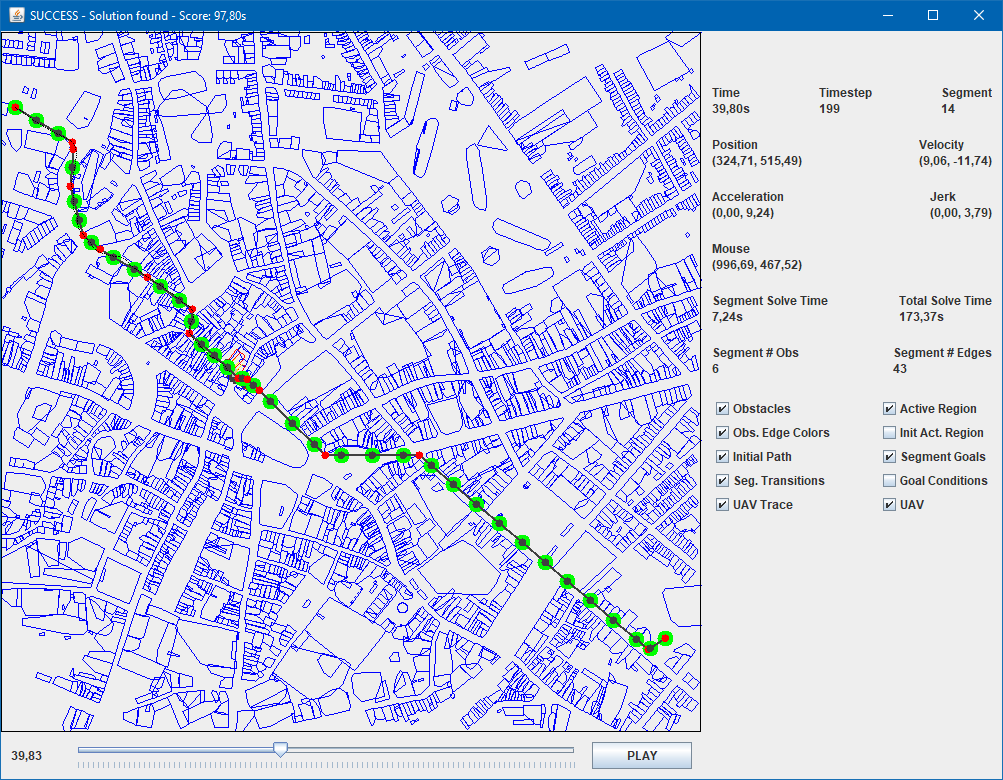
\includegraphics[width=\textwidth]{ui-full}
    \caption[An overview of the visualization tool]{An overview of the visualization tool that shows the results of the algorithm.}
    \label{fig:ui-full}     
\end{figure}
For this reason, I spent a significant amount of time building a visualization tool which displays not only the solution, but also the constraints of the MILP problem and other debugging information. This proved to be a critical part of the development cycle of the algorithm. Figure \ref{fig:ui-full} on page \pageref{fig:ui-full} shows this tool. At first glance, the tool may look familiar. It has been used to create many of the examples shown in this thesis. 
\subsection{Interface Elements}
The graphical interface is divided into three parts.

\paragraph{World view}The first and most prominent part is the visualization on the left. This shows a view of the world with a variety of information overlaid on top of it. The view can be translated by holding down the left mouse button and dragging around. Scrolling zooms in and out on the view.

\paragraph{Timeline}The second element is the timeline on the bottom. By dragging the slider, the user can change the time step being visualized. There is also a play/pause button which can be used to animate the visualization. The animation runs in real-time according to the progress of time of the trajectory. The animations help spot more subtle changes in acceleration which are not immediately clear from the still view.

\paragraph{Data Panel} The last element is the panel on the right. This panel contains more detailed information about the current time step being visualized. This information includes:
\begin{itemize}
\item The current time in the trajectory
\item The current time step number
\item The current segment number
\item The position, velocity, acceleration and jerk (derivative of acceleration) at the current time step
\item The world coordinates at the position of the mouse
\item The solve time for the current segment
\item The total execution time of the entire algorithm
\item The amount of obstacles and edges being modeled in the current segment
\end{itemize}
Along with that information, there are also visibility toggles for the various elements of the visualization.

\subsection{World View Elements}
\begin{figure}
	\centering
    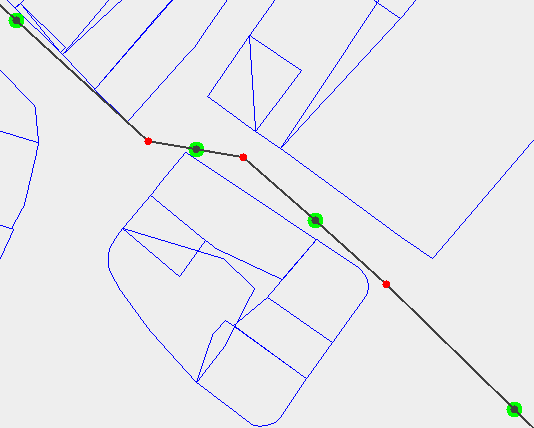
\includegraphics[width=0.7\textwidth]{vis-1}
    \caption[Visualization of the obstacles, initial path, turn events and segment goals]{The obstacles are blue, initial path is black with turn events being red. The green circles are the segment goals.}
    \label{fig:vis-1}     
\end{figure}
\paragraph{Obstacles} The obstacles are the most common element in the visualization. Obstacles are visualized as blue polygons. See Figure \ref{fig:vis-1}.
\paragraph{Initial path} The initial path is the result of the Theta* algorithm. It is shown as black lines. The turn events on this path are red. When multiple nodes on the path belong to the same turn event, the lines connecting them are also red. See Figure \ref{fig:vis-1}.
\paragraph{Segment goals} The segment goals are visualized as the green circles on the initial path. These goals mark both the end of a segment and the start of the next segment. See Figure \ref{fig:vis-1}.

\clearpage
\begin{figure}[h]
	\centering
    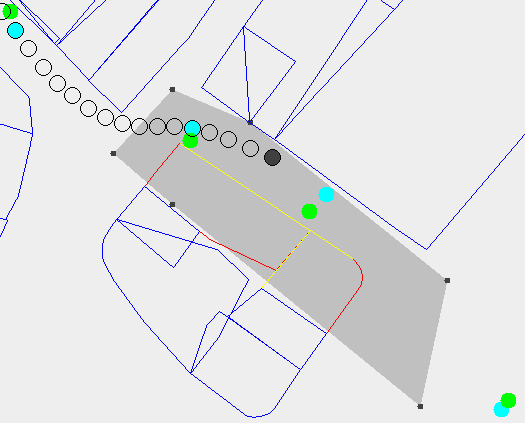
\includegraphics[width=0.7\textwidth]{vis-2}
    \caption[Visualization of the safe region, obstacle edge constrain state and the segment transitions.]{The safe region is dark grey and the segment transitions are the blue circles. The edges of the obstacles inside the safe region are yellow or red to signify whether or not the UAV is on the safe size of that edge.}
    \label{fig:vis-2}     
\end{figure}

\paragraph{Safe region} The safe region for the current segment, as generated by the genetic algorithm, is shows as a dark grey polygon. The UAV must stay within this polygon at all times. See Figure \ref{fig:vis-2}.
\paragraph{Obstacle Edge Colors} The obstacles within the safe region are modeled in the MILP problem. The color of the edges of these obstacles display whether or not the constraint is active for that edge at the current time step. If the color is yellow, the UAV is on the safe side of that edge. Otherwise, the color is red. See Figure \ref{fig:vis-2}.
\paragraph{Segment Transitions} The segment transitions do not always happen right at the goal positions of the segments. The blue circle shows the position of the UAV at the time of the actual segment transition. See Figure \ref{fig:vis-2}.
\newpage
\begin{figure}
	\centering
    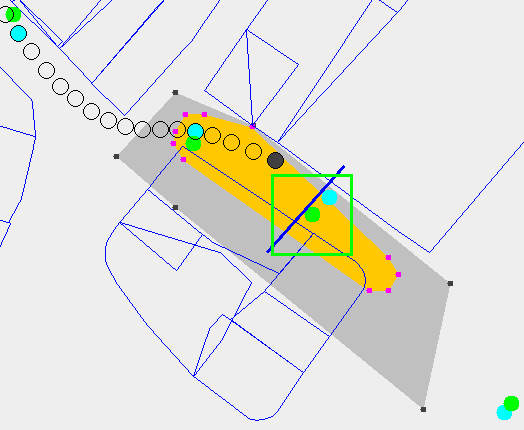
\includegraphics[width=0.7\textwidth]{vis-3}
    \caption[Visualization of the initial safe region and the segment goal conditions]{The initial safe region is shown in orange. To reach its goal, the UAV must be inside the green square and have crossed the blue finish line.}
    \label{fig:vis-3}     
\end{figure}

\paragraph{Initial Safe Region} Before the genetic algorithm is executed, an initial safe region is constructed which ensures the UAV can reach its goal in the current segment. This initial safe region is shown in orange. The (expanded) safe region from the genetic algorithm must completely contain this initial region. See Figure \ref{fig:vis-3}.
\paragraph{Goal Conditions} The UAV does not have to reach its goal exactly. The green square around the segment goal shows the tolerance region where the UAV is close enough to its goal. The blue line shows the finish line which the UAV must cross as well. See Figure \ref{fig:vis-3}.

